
\chapter{The standard model of particle physics}\label{sec:SM}
\textit{This chapter introduces the standard model (SM) of particle physics which describes the family of elementary particles and their interactions.}
\section{The elementary particles}\label{subsec:elem_particle}
It has been long time for people try to understand what is the basic object which constitutes our world. From Demokritos (~470-380 BC) who thought matter was built of discrete building blocks to John Dalton (1766-1844) who came up with the matter was made of atoms. In the early 1900's J.J. Thomson proposed a so called "plum pudding model" which assume the atom was a uniform sphere of positively charged matter in which electrons were embedded. However in 1910 Ernest Rutherford and his colleagues performed $\alpha$ rays scattering experiments and found that the whole mass and all positive charge of the atom were concentrated in a minute space at the centre which is called "nucleus". After the discovery of the neutron in 1932 by James Chadwick, models for a nucleus composed of protons and neutrons were quickly developed by Dmitri Ivanenko and Werner Heisenberg. Furthermore in 1968 the deep inelastic scattering experiments at the Stanford Linear Accelerator Center provided the first convincing evidence of the reality of quarks in the proton or neutron. In the standard model (SM) the quarks are the elementary particles and there are six different kinds of flavors for the quarks called up (u), down (d), charm (c), strange (s), top (t) and bottom (b), the mass, charge and spin of the quarks are shown in table \ref{tab:quarks}, here the $e$ means one electron's charge which equal $\mathrm{1.6\times10^{-19}C}$. The quarks are categorized in there generations which will be discussed in section \ref{subsubsec:strong_interaction}. Besides the quarks have another property which is called the "color charge", a quark can be "Red" or "Blue" or "Green". The reason for there are only three kinds of color charges will be discussed in section \ref{subsubsec:strong_interaction}. Moreover all the quarks have its anti-quark which has opposite quantum number with regard to quark including flavor, charge and color charge quantum number. Therefore there are $\mathrm{6~(flavor)~\times~3~(color)~\times~2(anti-quark)~=~36}$ kinds of quarks in the SM and all the hadrons are composed by quarks or anti-quarks, for meson it is composed by $\mathrm{q\bar{q}}$ and for baryon it is composed by $\mathrm{qqq}$ or $\mathrm{\bar{q}\bar{q}\bar{q}}$.
 \begin{table}[!hbpt]
 \begin{center}
 \begin{tabular}{|c|c|c|c|c|}
 \hline
 Generation           & Quark         & Charge      &Spin      & Mass \\ \hline
 First                & up quark (u)  & 2/3 $e$     &1/2       & $2.3^{+0.7}_{-0.5}$ MeV \\
                      & down quark (d)& -1/3 $e$    &1/2       & $4.8^{+0.5}_{-0.3}$ MeV \\ \hline
 Second               & charm quark (c)& 2/3 $e$    &1/2       & $1.275 \pm 0.025$ GeV \\
                      & strange quark (s)& -1/3 $e$ &1/2       & $95\pm 5$ MeV \\  \hline
 Third                & top quark (t)    & 2/3 $e$  &1/2       & $173.21\pm 0.51 \pm 0.71$ GeV \\
                      & bottom quark (b) & -1/3 $e$ &1/2       & $4.66 \pm 0.03$ GeV \\ \hline
 \end{tabular}
 \end{center}
 \caption{Quarks and their properties \cite{Olive:2016xmw}.\label{tab:quarks}}
 \end{table}

Similar with quark family there are a lepton family, the most common one is electron which exists as a cloud out of nucleus to form an atom. All the leptons are shown in table \ref{tab:leptons} with their charge, spin and mass, they are electron ($\mathrm{e}$), electron neutrino ($\mathrm{\nu_e}$), muon ($\mathrm{\mu}$), muon neutrino ($\mathrm{\nu_{\mu}}$), tau ($\mathrm{\tau}$) and tau neutrino ($\mathrm{\nu_{\tau}}$). The leptons are also categorized into three generations and each generation has its own lepton flavor. First generation are electron flavor leptons, second generation are muon flavor leptons and third generation are tau flavor leptons. The reason for neutrinos have non-zero mass is because of the observation of neutrino's oscillations otherwise in SM the mass of neutrinos are zero. Similar with the quarks, all the leptons also have theirs anti-particle partners which own the opposite quantum number. While unlike the quarks, the leptons do not have color charge property. Therefore there are $6~\times~2~=~12$ kinds of leptons in SM.

Now the all the spin 1/2 (fermion) elementary particles in SM are introudced, in section \ref{subsec:fund_interaction} the interactions between these particles and the mediators will be discussed.

\begin{table}[!hbpt]
\begin{center}
\begin{tabular}{|c|c|c|c|c|}
\hline
Generation & Lepton                               & Charge &Spin & Mass \\ \hline
First      & electron ($\mathrm{e}$)              & -$e$   &1/2  & 511 MeV\\
           & electron neutrino ($\mathrm{\nu_e}$) & 0      &1/2  & $<$ 2 eV\\ \hline
Second     & muon ($\mathrm{\mu}$)                & -$e$   &1/2  & 105.67 MeV\\
           & muon neutrino ($\mathrm{\nu_{\mu}}$) & 0      &1/2  & $<$ 2 eV\\ \hline
Third      & tau ($\mathrm{\tau}$)                & -$e$   &1/2  & 1776.99 MeV\\
           & tau neutrino ($\mathrm{\nu_{\tau}}$) & 0      &1/2  & $<$ 2 eV\\ \hline
 \end{tabular}
 \end{center}
 \caption{Properties of the leptons in the three generations. Neutrinos are assumed to have zero mass in SM but by the observation of neutrino's oscillations the upper limits on their mass are set\cite{Olive:2016xmw}.\label{tab:leptons}}
 \end{table}

\section{The fundamental interactions}\label{subsec:fund_interaction}
It is well known there are four characteristic interactions among fundamental particles.
\begin{enumerate}
\item Electromagnetic interaction : It is mediated by massless photon ($\mathrm{m_{\gamma}~=~0}$) with spin = 1 among charged particles. Because of the massless of photon the interacting range of electromagnetic interaction is infinite. The theory to describe the electromagnetic interaction is quantum electrodynamics (QED) which is well understood.  QED is renormalizable for example the divergence from vacuum polarization and higher order loop contributions can be absorbed in to the physical charge of particle. The coupling constant is $\mathrm{\alpha~=~\frac{e^{2}}{4\pi\varepsilon_{0}\hbar c}} ~\simeq ~ \frac{1}{137}$ which characterizes the strength of the coupling of charged particle with the electromagnetic field. Because of smallness of $\mathrm{\alpha}$ the perturbation works well for QED. Besides the $\mathrm{\alpha}$ is running coupling which means it will increase when the energy scale of interaction increase, but the difference is very small for wide energy scale.
\item Weak interaction : It is mediated by massive weak bosons ($\mathrm{m_{W^{\pm}}~\cong~80.4~GeV/c^{2},}$ \\ $\mathrm{m_{Z}~\cong~91.2~GeV/c^{2}}$) with spin = 1 because of the heavy mediator its interacting range is very short which is $\sim 10^{-18}?$. The coupling strength of weak interaction is the weakest among electromagnetic and strong interactions which is $\sim 10^{-14}?$. Although the coupling strength is small, some process can only happen via weak interaction like flavor changing or neutrino involved
    processes.
\item Strong interaction : It is mediated by massless gluons ($\mathrm{m_{g}~=~0}$) with spin = 1. This interaction can only happen between quarks and gluons. The theory describes the strong interaction is called quantum chromodynamics (QCD). For strong interaction the coupling strength is also running but opposite with electromagnetic interaction which means the coupling will decrease when the interaction energy increase. Because of that there are one special phenomenon for strong interaction called "asymptotic free" which means quarks and gluons behaviour like free particle when the interaction energy is very high. In high energy the perturbation theory works because of "asymptotic free" but not for low energy which is few hundred $\mathrm{MeV}$. Therefore there are a still lot of works need to be done for describing QCD process in low energy. Another special phenomenon for strong interaction is called the "color confinement", which means there are no free quarks in the world, all quarks need other quarks to form a colorless hadron for instance the baryon is formed by red, green and blue quarks or the meson is formed by red and anti-red quarks or blue and anti-blue quarks or green and anti-green quarks.
\item Gravitational interaction : It is mediated by massless gravitons ($\mathrm{m_{G}~=~0}$) with spin = 2 among all massive particles. Because of its very samll coupling strength we normally do not consider gravitational interaction in high energy physics. For macroscopic world the gravitation is important like it makes an apple falling.
\end{enumerate}

The summary of interaction range, mediator and relative strength for four fundamental interactions is shown in \ref{tab:interactions}.
Last but not least in standard model the origin of mass of the particles is coming from interaction between particles and a scalar field which is known the Brout-Englert-Higgs scalar boson. In 2012 the ATLAS \cite{Aad:2012tfa} and CMS \cite{Chatrchyan:2012xdj} experiments observed such a particle and the mass is $\sim \mathrm{125 GeV}$.

The summary of all elementary particles, force carries and Brout-Englert-Higgs boson is shown in \ref{fig:SM}.

 \begin{table}[!hbpt]
 \begin{center}
 \begin{tabular}{|c|c|c|c|}
 \hline
 Interaction & Range & Relative strength & Mediators \\
 \hline
 Strong & $10^{-15}$ m & 1 &  8 gluons ($g$) \\
 \hline
 Electromagnetic & $\infty$ & $10^{-3}$ & photon ($\gamma$) \\
 \hline
 Weak &  $10^{-18}$ m & $10^{-14}$ & $\mathrm{W^+}$, $\mathrm{W^-}$, $\mathrm{Z}$ \\
 \hline
 Gravitational & $\infty$ & $10^{-43}$ & graviton (G) ? \\
 \hline
  \end{tabular}
 \end{center}
 \caption{Range, relative strength with respect to the strong force, and mediators of the four fundamental interactions. The gravitational force is not included in the SM, and gravitons are hypothetical particles.
 \label{tab:interactions}
}
 \end{table}

\begin{figure}[h!]
 \begin{center}
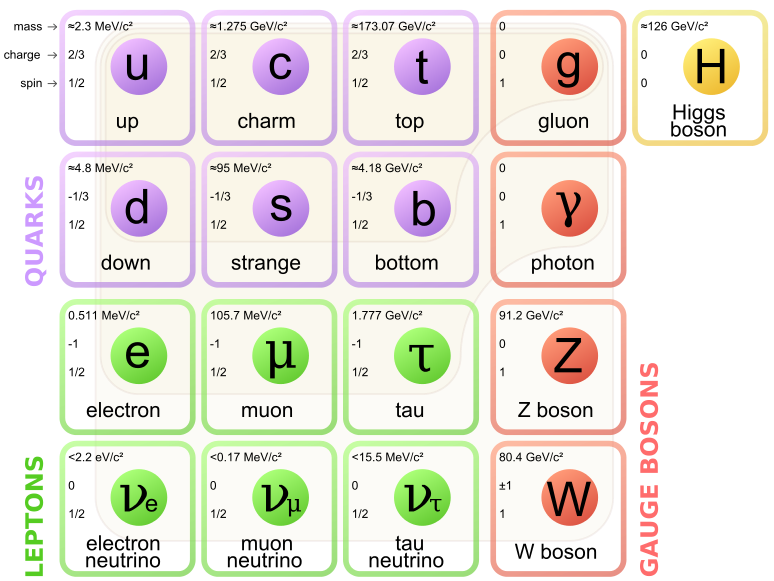
\includegraphics[width=0.75\textwidth]{figures/theory/sm.png}
\caption{Overview of the Standard Model constituents.}
  \label{fig:SM}
 \end{center}
\end{figure}

\section{The feynman calculus}\label{subsec:Feynman}
\subsection{Lifetimes}\label{subsubsec:Lifetime}
As we know all particles can be separated by two categories, one is stable particle another is unstable particle. Such as the electron, photon and proton which are stable, while the muon, tau and neutron which are unstable. Actually most of particles are unstable and we are interested in what is the mass, lifetime, decay channel, spin and so on of these particles.
For the unstable particles the number of particle versus time can be expressed by \ref{eq:Nt} which comes from the integration of \ref{eq:dN}, here the $\Gamma$ means the decay rate of the particle and $\tau~=~\frac{1}{\Gamma}$ is called the mean lifetime of the particle.
\begin{equation}
N(t)~=~N(0)e^{-\Gamma t}
\label{eq:Nt}
\end{equation}
\begin{equation}
dN~=~-\Gamma~N~dt
\label{eq:dN}
\end{equation}
Moreover if the particle can decay by different channels then each channel has different decay rate so the total decay rate is the sum of decay rate of each channel which is shown in \ref{eq:Gammatot}.
\begin{equation}
\Gamma_{tot}~=~\sum^{n}_{i=1}~\Gamma_{i}
\label{eq:Gammatot}
\end{equation}
In addition to $\tau$, we want to calculate the branching ratios which is the fraction of total particles decay to each channel. It is determined by the decay rates showed in \ref{eq:Bri}.
\begin{equation}
Br_{i}~=~\frac{\Gamma_{i}}{\Gamma_{tot}}
\label{eq:Bri}
\end{equation}
Therefore the most important physical quantity to describe the decay is the $\Gamma$ and the way to calculate it will be described in section \ref{subsubsec:golden_rule}.

Actually using the Schr$\mathrm{\ddot{o}}$dinger equation (the \ref{eq:Schro}) the wave function of the decay particle can be expressed by \ref{eq:wave}, the $E_{R}$ is the energy of the particle. And the existence possibility of the particle versus time is $\Psi\Psi^{\ast}\varpropto e^{\Gamma t}$ which is consistent with \ref{eq:Nt}.
\begin{equation}
(\frac{-\hbar^{2}}{2m}\nabla^{2}~+~ V)\Psi~=~i\hbar\frac{\partial}{\partial t}~\Psi ~~~~(\mathrm{Schr\ddot{o}dinger~equation})
\label{eq:Schro}
\end{equation}
\begin{equation}
\Psi(t)~=~\Psi(0)e^{-iE_{R}t}e^{\frac{-t}{2\tau}},~\mathrm{here~the}~\hbar~=~c~=~1
\label{eq:wave}
\end{equation}
Using Fourier transform we can represent the wave function as the function of energy which is shown in \ref{eq:Fourier}.
\begin{equation}
\chi(E)~=\int_{0}^{+\infty}~\Psi(t)e^{iEt}dt=\Psi(0)\int_{0}^{+\infty}e^{-t[\frac{\Gamma}{2}+i(E_{R}-E)]}dt~=~\frac{\Psi(0)}{(E-E_{R})-\frac{i\Gamma}{2}}
\label{eq:Fourier}
\end{equation}
Finally the existence possibility of the particle versus energy is $\chi\chi^{\ast}$ which is shown in \ref{eq:wave_BW} and it gives the form of non-relativistic Breit Wigner (BW) distribution. Using the particle itself as the reference frame we can replace the $E_{R}$ by $M_{R}$ which is the mass of the particle. The full wave at half maximum (FWHM) of BW distribution is the $\Gamma$.
\begin{equation}
\chi(E)\chi(E)^{\ast}~=\frac{\Psi(0)\Psi(0)^{\ast}}{(E-E_{R})^{2}+\frac{\Gamma^{2}}{4}}
\label{eq:wave_BW}
\end{equation}
\subsection{Cross section}\label{subsubsec:Cross_section}
One very important physical quantity in high energy physics is "cross section". The cross section characterize the possibility of one physical process will be happen and its unit is $\mathrm{cm^{-2}}$. For example for electron elastic scattering process $\mathrm{e~+~e\rightarrow~e~+~e}$ if we know the cross section $\sigma$ and the luminosity $\mathcal{L}$ which means the number of $\mathrm{e~e}$ scattering (include elastic and inelastic) events in one $\mathrm{cm^{2}}$ then the number of $\mathrm{e~e}$ elastic scattering events can be expressed by \ref{eq:N_elastic}.
\begin{equation}
N_{elastic}=\sigma_{elastic}*\mathcal{L}
\label{eq:N_elastic}
\end{equation}
If we want to measure the cross section of $\mathrm{e~e}$ scattering for all possible process like $\mathrm{e~+~e\rightarrow anything}$, then it equal sum of the cross section for each process.
\begin{equation}
\sigma_{tot}=\sum_{i=1}^{n}\sigma_{i}
\label{eq:sigma_tot}
\end{equation}
The way to calculate the cross section is explained in \ref{subsubsec:golden_rule}.
\subsection{The golden rule}\label{subsubsec:golden_rule}
The transition rate for a given process is described by the Fermi's "Golden Rule" shown in \ref{eq:golden_rule}. The $\mathcal{M}$ is called the amplitude for the process which contains all the dynamical information and it can be calculated by evaluating the relevant Feynman diagrams using the "Feynman rules". The phase space factor contains only the kinematical information, it depends on the masses, energies and momenta of the participants. For example a heavy particle decay into many light particles will involves a large phase space factor because there are many ways to apportion the available energy. By contrast, the decay of neutron ($\mathrm{n~\rightarrow~p~+~e+~\bar{\nu_{e}}}$) has very small phase space for the final state particles because the proton's mass just a bit smaller than neutron's.
\begin{equation}
\mathrm{transition~rate~=~\frac{2\pi}{\hbar}~|\mathcal{M}|^{2}~*~(phase~space)}
\label{eq:golden_rule}
\end{equation}
\begin{itemize}
\item[$\bullet$] The golden rule for decay.
 Suppose one particle decays into several other particles:
 \begin{equation}
 1~\rightarrow~2~+~3+~...~+~n
 \label{eq:one_decay}
\end{equation}
 The decay rate is given by the formula \ref{eq:golden_rule_decay}. Here the $p_{i}~=~(E_{i}/c,\mathbf{p_{i}})$ is the four-momentum of the $i$th particle with $m_{i}^{2}c^{4}~=~E_{i}^{2}~-~\mathbf{p_{i}^{2}c^{2}}$. The $\delta$ function enforces conservation of energy and momentum between decaying particle and final state particles. The decaying particle is assumed to be at rest so the $p_{1}~=~(m_{1}c^{2},\mathbf{0})$. the $S$ is equal $\frac{1}{j!}$ for each group of $j$ identical particles in the final state.
\begin{equation}
d\Gamma~=~|\mathcal{M}|^{2}~\frac{S}{2\hbar m_{1}}~[(\frac{c~d^{3}\mathbf{p_{2}}}{(2\pi)^{3}2E_{2}})(\frac{c~d^{3}\mathbf{p_{3}}}{(2\pi)^{3}2E_{3}})~...~(\frac{c~d^{3}\mathbf{p_{n}}}{(2\pi)^{3}2E_{n}})]\\
*(2\pi)^{4}\delta^{4}(p_{1}~-~p_{2}~-~p_{3}~...~-p_{n})
\label{eq:golden_rule_decay}
\end{equation}
The equation \ref{eq:golden_rule_decay} is the differential rate for a decay in which the momentum of particle 2 is within the range $d^{3}\mathbf{p_{2}}$ about the value $\mathbf{p_{2}}$, similar for other final state particles. Usually we are more interested in the decay rate for full phase space of final state particles, so we can integrate the equation \ref{eq:golden_rule_decay} over all momenta of final state particles to get the total decay rate $\Gamma$. For example for two body decay the total $\Gamma$ is expressed in \ref{eq:golden_rule_decay_int}, besides after some algebraic calculations the equation \ref{eq:golden_rule_decay_int} can be simplified with equation \ref{eq:golden_rule_decay_simp} and without knowing $\mathcal{M}$ which is the function of final state particles momenta. Here the $\mathbf{p}$ is the magnitude of momentum for either final state particle. However there are no such simplified equation for more than two body decay until we know the specific functional from of $\mathcal{M}$. In such case we can only go back to the equation \ref{eq:golden_rule_decay} and work it out from scratch.
\begin{equation}
\Gamma~=~\frac{S}{\hbar m_{1}}~(\frac{c}{4\pi})^{2}~\frac{1}{2}~\int\frac{|\mathcal{M}|^{2}}{E_{2}E_{3}}~\delta^{4}(p_{1}~-~p_{2}~-~p_{3})~d^{3}\mathbf{p_{2}}d^{3}\mathbf{p_{3}}
\label{eq:golden_rule_decay_int}
\end{equation}
\begin{equation}
\Gamma~=~\frac{S|\mathcal{M}|^{2}|\mathbf{p}|}{8\pi\hbar m_{1}^{2}c},~|\mathbf{p}|~=~\frac{c}{2m_{1}}\sqrt{m_{1}^{4}~+~m_{2}^{4}~+~m_{3}^{4}~-~2m_{1}^{2}m_{2}^{2}~-~2m_{1}^{2}m_{3}^{2}~-~2m_{2}^{2}m_{3}^{2}}
\label{eq:golden_rule_decay_simp}
\end{equation}

\item[$\bullet$] The golden rule for scattering.
 Suppose two particles collide and producing several particles:
 \begin{equation}
1~+~2~\rightarrow~3~+~4~+~...~+~n
 \label{eq:two_scat}
\end{equation}
The cross section is given by the formula \ref{eq:golden_rule_scat}. Here, as before, the $p_{i}~=~(E_{i}/c,\mathbf{p_{i}})$ is the four-momentum of the $i$th particle with $m_{i}^{2}c^{4}~=~E_{i}^{2}~-~\mathbf{p_{i}^{2}c^{2}}$. The $\delta$ function enforces conservation of energy and momentum. the $S$ is equal $\frac{1}{j!}$ for each group of $j$ identical particles in the final state.
\begin{equation}
\begin{split}
d\sigma~=&~|\mathcal{M}|^{2}~\frac{\hbar^{2}S}{4\sqrt{(p_{1}\cdot p_{2})^{2}-(m_{1}m_{2}c^{2})^{2}}}[(\frac{c~d^{3}\mathbf{p_{3}}}{(2\pi)^{3}2E_{3}})(\frac{c~d^{3}\mathbf{p_{4}}}{(2\pi)^{3}2E_{4}})~...~(\frac{c~d^{3}\mathbf{p_{n}}}{(2\pi)^{3}2E_{n}})]\\
&*(2\pi)^{4}\delta^{4}(p_{1}~+~p_{2}~-~p_{3}~-~p_{4}~...~-p_{n})
\end{split}
\label{eq:golden_rule_scat}
\end{equation}
Equation \ref{eq:golden_rule_scat} gives the cross section when the momentum of particle 3 within the range $d^{3}\mathbf{p_{3}}$ about the value $\mathbf{p_{3}}$, similar for other final state particles. If we want to know the total cross section for full phase space, we can integrate the equation over the momenta of all particles.
Similar with decay, for two body scattering ($1~+~2~\rightarrow~3~+~4$) in the central mass (CM) frame we can get simplified equation which is shown in \ref{eq:golden_rule_scat_two}. Here the $|\mathbf{p_{i}}|$ is the magnitude of either incoming momentum and $|\mathbf{p_{f}}|$ is the magnitude of either outgoing momentum, the $d\Omega~=~sin\theta~d\theta~d\phi$ is the differential solid angle of either outgoing particle. For more than two body scattering we need work it out from scratch using equation \ref{eq:golden_rule_scat}.
\begin{equation}
\frac{d\sigma}{d\Omega}~=~(\frac{\hbar c}{8\pi})^{2}~\frac{S|\mathcal{M}^{2}|}{(E_{1}~+~E_{2})^{2}}~\frac{|\mathbf{p_{f}}|}{|\mathbf{p_{i}}|}
\label{eq:golden_rule_scat_two}
\end{equation}
\end{itemize}

Now we know the form of golden rule for calculating the decay rate and scattering cross section, while in order to get the exact value we still need to know the $\mathcal{M}$ in the equations and it can be calculated by evaluating the relevant Feynman diagrams using the "Feynman rules" which is explained in section \ref{subsubsec:feynman_toy}.

\subsection{The Feynman rules for a toy theory}\label{subsubsec:feynman_toy}
This section will gives the Feynman rules for a toy theory which means the spin of the particles are not considered, so it will not present the real world which is more complicated and will be addressed in section, but still it gives the basic idea how Feynman rules works. Below is the ritual:
\begin{enumerate}
\item $\mathbf{Draw~the~Feynman~diagram:}$ The figure \ref{fig:feynman_decay_scatter} shows an example of the lowest-order Feynman digram for particle $A$ decay into particle $B$ and $C$ in the left plot and two particles scattering ($A~+~A~\rightarrow~B~+~B$) in the right. The $p_{i}$ means the four-momenta of incoming or outgoing particles, the $q_{i}$ means the four-momenta of intermediate particles like the particle $C$ in the right plot of \ref{fig:feynman_decay_scatter}. The arrow on each line represent the direction of the particle's movement (for internal lines it is arbitrary).
\begin{figure}[h!]
 \begin{center}
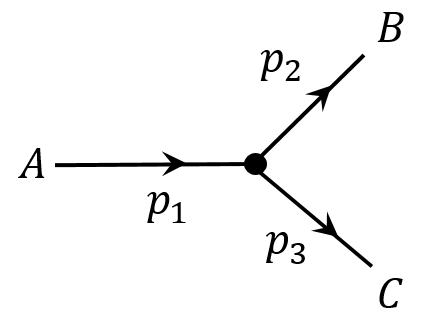
\includegraphics[width=0.4\textwidth]{figures/theory/feynman_decay.png}
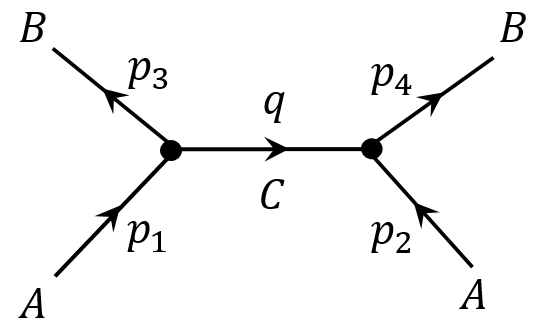
\includegraphics[width=0.45\textwidth]{figures/theory/feynman_scatter.png}
\caption{The lowest-order Feynman diagram for $A~\rightarrow~B~+~C$ (left) and $A~+~A~\rightarrow~B~+~B$ (right).}
  \label{fig:feynman_decay_scatter}
 \end{center}
\end{figure}
\item $\mathbf{Coupling~Constant:}$ For each vertex write down a factor of $-ig$. The $g$ is called coupling constant which represent the strength of the interaction between different particles.
\item $\mathbf{Propagator:}$ For each internal line write down a factor of $\frac{i}{q^{2}_{i}-m_{i}^{2}c^{2}}$, here the $q_{i}$ is the four-momentum of the line ($q_{i}^{2}~=~(\frac{E_{i}}{c})^{2}~-~\mathbf{p_{i}}^{2}$) and the $m_{i}$ is the rest mass of the particle the internal line describes. Note that $q_{i}^{2}~\neq~m_{i}^{2}c^{2}$, because the propagator is virtual particle and it does not lie on its mass shell.
\item $\mathbf{Conservation~of~energy~and~momentum:}$ For each vertex write down a $\delta$ function with the form of $(2\pi)^{4}\delta^{4}(k_{1}~+~k_{2}~+~k_{3})$. Here the $k_{i}$ are the four-momentum of the particle which involved in the vertex, if the arrow of line $k_{i}$ is toward to the vertex then put a positive sign in front of $k_{i}$ otherwise put a negative sign. This factor imposes the conservation of energy and momentum at each vertex, since the $\delta$ function is zero unless the sum of incoming momenta equals the sum of outgoing momenta.
\item $\mathbf{Integration~over~internal~momenta:}$ For each internal line write down a factor $\frac{1}{(2\pi)^{4}d^{4}q_{i}}$ and integrate over all internal momenta.
\item $\mathbf{Cancel~the~\delta~function:}$ Erase $(2\pi)^{4}\delta^{4}(p_{1}~+~p_{2}~+~...~+~p_{n})$ in the result which enforcing overall conservation of energy and momentum. Finally what remains is $-i\mathcal{M}$.
\end{enumerate}

Now we can use Feynman rules to get the amplitude for lowest-order of particle $A$ decay into particle $B$ and $C$ (see figure \ref{fig:feynman_decay_scatter} left). Through rule 1 to 5 it gives $(-ig)(2\pi)^{4}(p_{1}~-~p_{2}~-~p_{3})$ and using rule 6 it remains $-ig$ only which equal $-i\mathcal{M}$. Finally the $\mathcal{M}$ equal $g$.
Therefore the decay rate of particle $A$ is found by plugging $\mathcal{M}$ into equation \ref{eq:golden_rule_decay_simp} which is shown in \ref{eq:decay_rate_two}.
The lifetime of the particle $A$ is shown in \ref{eq:lifetime_two}.
\begin{equation}
\Gamma~=~\frac{g^{2}|\mathbf{p}|}{8\pi\hbar m_{A}^{2}c},~|\mathbf{p}|~=~\frac{c}{2m_{A}}\sqrt{m_{A}^{4}~+~m_{B}^{4}~+~m_{C}^{4}~-~2m_{A}^{2}m_{B}^{2}~-~2m_{A}^{2}m_{C}^{2}~-~2m_{B}^{2}m_{C}^{2}}
\label{eq:decay_rate_two}
\end{equation}
\begin{equation}
\tau~=~\frac{1}{\Gamma}~=~\frac{8\pi\hbar m_{A}^{2}c}{g^{2}|\mathbf{p}|}
\label{eq:lifetime_two}
\end{equation}
Similarly using Feynman rules we can get the amplitude for lowest-order of two particles $A$ scattering process $A~+~A~\rightarrow~B~+~B$ (shown in figure \ref{fig:feynman_decay_scatter} right). The result of rule 1 to rule 5 is shown in \ref{eq:scat_amplidted15}. After some algebraic calculations and using rule 6, the final result for $\mathcal{M}$ is shown in \ref{eq:scat_amplidted}.
\begin{equation}
\begin{split}
\int(-ig)^{2}~\frac{i}{q^{2}-m_{C}^{2}c^{2}}~(2\pi)^{4}\delta^{4}(p_{1}-p_{3}-q)~(2\pi)^{4}\delta^{4}(p_{2}+q-p_{4})~\frac{1}{(2\pi)^{4}}d^{4}q
\end{split}
\label{eq:scat_amplidted15}
\end{equation}
\begin{equation}
\mathcal{M}~=~\frac{g^{2}}{(p_{1}-p_{3})^{2}-m_{C}^{2}c^{2}}~=~\frac{g^{2}}{(p_{4}-p_{2})^{2}-m_{C}^{2}c^{2}}
\label{eq:scat_amplidted}
\end{equation}

But there is another diagram contribute to the lowest-order of the process ($A~+~A~\rightarrow~B~+~B$) which is shown in figure \ref{fig:feynman_scatter_2}. This is obtained by twisting the outgoing lines of the right plot of figure \ref{fig:feynman_decay_scatter} and making $p_{1}$ connect to $p_{4}$, $p_{2}$ connect to $p_{3}$. Similar we can using Feynman rules to get the amplitude for this process. Finally sum up the $\mathcal{M}$ form these two lower-order diagram, we can get the total $\mathcal{M}$ for $A~+~A~\rightarrow~B~+~B$ processes which is shown in \ref{eq:scat_amplidted_tot}.
\begin{figure}[h!]
 \begin{center}
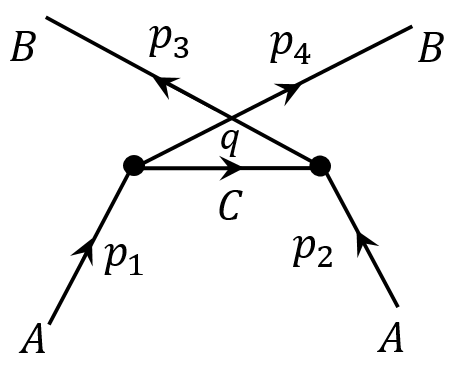
\includegraphics[width=0.45\textwidth]{figures/theory/feynman_scatter_2.png}
\caption{Another Feynman diagram contributing in lowest-order to $A~+~A~\rightarrow~B~+~B$.}
  \label{fig:feynman_scatter_2}
 \end{center}
\end{figure}
\begin{equation}
\mathcal{M}~=~\frac{g^{2}}{(p_{1}-p_{3})^{2}-m_{C}^{2}c^{2}}~+~\frac{g^{2}}{(p_{3}-p_{2})^{2}-m_{C}^{2}c^{2}}
\label{eq:scat_amplidted_tot}
\end{equation}

\clearpage
%%%%%%%%%%%%%%%%%%% QED%%%%%%%%%%%%%%%%%%%%%%%%%%%%%%%%%%%
\section{Quantum Electrodynamics}\label{subsec:QED}
Here we are going to introduce some basic knowledge of Quantum Electrodynamics (QED) including the Dirac equation, the photon wavefunction and the Feynman rules for QED.
\subsection{Dirac equation}\label{subsec:Dirac}
As we know in nonrelativistic quantum mechanics particles are described by the Schr$\mathrm{\ddot{o}}$dinger equation (the \ref{eq:Schro}). In relativistic quantum mechanics  particles of spin $\frac{1}{2}$ are described by Dirac equation which is shown in equation \ref{eq:Dirac} with the definition of $\partial_{\mu}$ \ref{eq:partial} and $\gamma^{\mu}$ \ref{eq:gamma_matrix} (the standard "Bjorken and Drell" convention). For particles with other spins such as spin 0 particles they are described by the Klein-Gordon equation \ref{eq:KG} and spin 1 particles are described by Proca equation.

\begin{equation}
i\hbar \gamma^{\mu}\partial_{\mu}\Psi-mc\Psi~=0 ~~\mathrm{(Dirac~equation)}
\label{eq:Dirac}
\end{equation}

\begin{equation}
\partial_{\mu}\equiv\frac{\partial}{\partial x^{\mu}},~
\partial_{0}=\frac{1}{c}\frac{\partial}{\partial t},~\partial_{1}=\frac{\partial}{\partial x},~\partial_{2}=\frac{\partial}{\partial y},~\partial_{3}=\frac{\partial}{\partial z}
\label{eq:partial}
\end{equation}

\begin{equation}
\begin{split}
&\gamma^{0}=\begin{pmatrix} 1 & 0 \\ 0 & -1 \end{pmatrix},~
\gamma^{i}=\begin{pmatrix} 0 & \sigma^{i} \\ -\sigma^{i} & 0 \end{pmatrix} \\
&\sigma^{1}=\begin{pmatrix} 0 & 1 \\ 1 & 0 \end{pmatrix},~\sigma^{2}=\begin{pmatrix} 0 & -i \\ i & 0 \end{pmatrix},~\sigma^{3}=\begin{pmatrix} 1 & 0 \\ 0 & -1 \end{pmatrix}
\end{split}
\label{eq:gamma_matrix}
\end{equation}

\begin{equation}
-\frac{1}{c^{2}}\frac{\partial^{2}\Psi}{\partial t^{2}}+\nabla^{2}\Psi~=(\frac{mc}{\hbar})^{2}\Psi ~~\mathrm{(Klein-Gordon~equation)}
\label{eq:KG}
\end{equation}

We can using Dirac equation to solve the plane wave function \ref{eq:plane_wave} of particles with spin $\frac{1}{2}$. Here the $a$ is normalization constant and $u(p)$ represent the spin of particles.
\begin{equation}
\Psi(x)~=~ae^{-(i/\hbar)x\cdot p}u(p),~\mathrm{with~x=(ct,\mathbf{x}),~p=(\frac{E}{c},\mathbf{p})}
\label{eq:plane_wave}
\end{equation}
Putting this into the Dirac equation \ref{eq:Dirac} it gives equation \ref{eq:plane_wave_s1} and using equation \ref{eq:plane_wave_s2} the we get \ref{eq:plane_wave_s3}.

\begin{equation}
(\gamma^{\mu}p_{\mu}-mc)u=0
\label{eq:plane_wave_s1}
\end{equation}
\begin{equation}
\gamma^{\mu}p_{\mu}=\gamma^{0}p_{0}-\pmb{\gamma}\cdot\mathbf{p}=\frac{E}{c}\begin{pmatrix} 1 & 0 \\ 0 & -1 \end{pmatrix}-\mathbf{p}\cdot \begin{pmatrix} 0 & \pmb{\sigma} \\ -\pmb{\sigma} & 0 \end{pmatrix}=\begin{pmatrix} E/c & -\mathbf{p}\cdot \pmb{\sigma} \\ \mathbf{p}\cdot \pmb{\sigma} & -E/c \end{pmatrix}
\label{eq:plane_wave_s2}
\end{equation}
\begin{equation}
(\gamma^{\mu}p_{\mu}-mc)u=\begin{pmatrix} \frac{E}{c}-mc & -\mathbf{p}\cdot \pmb{\sigma} \\ \mathbf{p}\cdot \pmb{\sigma} & -\frac{E}{c}-mc \end{pmatrix}\begin{pmatrix} u_{A} \\ u_{B} \end{pmatrix}=\begin{pmatrix} (\frac{E}{c}-mc)u_{A} -\mathbf{p}\cdot \pmb{\sigma}u_{B} \\ \mathbf{p}\cdot \pmb{\sigma}u_{A}-(\frac{E}{c}+mc)u_{B} \end{pmatrix}
\label{eq:plane_wave_s3}
\end{equation}
Finally after some algebraic calculations we get the two solutions for electron shown in \ref{eq:plane_wave_s4} and two solutions for positron shown in \ref{eq:plane_wave_s5} and the normalization constant $N=\sqrt{(|E|+mc^{2})/c}$ in order to satisfy the normalization requirement $u^{\dag}u=2|E|/c$.
\begin{equation}
u^{(1)}=N\begin{pmatrix} 1 \\ 0 \\ \frac{cp_{z}}{E+mc^{2}} \\ \frac{c(p_{x}+ip_{y})}{E+mc^{2}} \end{pmatrix},~
u^{(2)}=N\begin{pmatrix} 0 \\ 1 \\ \frac{c(p_{x}-ip_{y})}{E+mc^{2}} \\ \frac{-cp_{z}}{E+mc^{2}} \end{pmatrix}, \mathrm{with}~E=\sqrt{m^{2}c^{4}+\mathbf{p}^{2}c^{2}}
\label{eq:plane_wave_s4}
\end{equation}

\begin{equation}
u^{(3)}=N\begin{pmatrix} \frac{cp_{z}}{E-mc^{2}} \\ \frac{c(p_{x}+ip_{y})}{E-mc^{2}} \\ 1 \\ 0 \end{pmatrix},~
u^{(4)}=N\begin{pmatrix} \frac{c(p_{x}-ip_{y})}{E-mc^{2}} \\ \frac{-cp_{z}}{E-mc^{2}} \\ 0 \\ 1 \end{pmatrix}, \mathrm{with}~E=-\sqrt{m^{2}c^{4}+\mathbf{p}^{2}c^{2}}
\label{eq:plane_wave_s5}
\end{equation}

Moreover if we choose the direction of motion as Z axis then the $u^{(i)}$ will be the eigenstate of $S_{z}$ which is defined in \ref{eq:spin}, the $u^{(1)}$ and $ u^{(3)}$ are spin up, $u^{(2)}$ and $ u^{(4)}$ are spin down.
\begin{equation}
\mathbf{S}=\frac{\hbar}{2}\begin{pmatrix} \pmb{\sigma} & 0\\ 0 & \pmb{\sigma}\end{pmatrix}
\label{eq:spin}
\end{equation}

\subsection{The photon}\label{subsec:Photon}
As we know in classical electrodynamic theory the electric field ($\mathbf{E}$) and magnetic field ($\mathbf{B}$) is described by Maxwell's equations shown in \ref{eq:Maxwell} with charge density $\rho$ and current density $\mathbf{J}$.

\begin{equation}
\begin{split}
&(\mathbf{i})~~\nabla\cdot \mathbf{E}=4\pi\rho ~~~~~~~~~~~~ (\mathbf{iii})~~\nabla\cdot \mathbf{B}=0 \\
&(\mathbf{ii})~~\nabla\times\mathbf{E}+\frac{1}{c}\frac{\partial\mathbf{B}}{\partial t}=0 ~~(\mathbf{iv})~~\nabla\times\mathbf{B}-\frac{1}{c}\frac{\partial\mathbf{E}}{\partial t}=\frac{4\pi}{c}\mathbf{J}
\end{split}
\label{eq:Maxwell}
\end{equation}

If we using the "field strength tensor" $F^{\mu\nu}$ shown in \ref{eq:F_tensor} (e.g. $F^{01}=-E_{x}, ~F^{12}=-B_{z}$, etc.) and $J^{\mu}$ show in \ref{eq:J_mu} then the equation $\mathbf{i}$ and $\mathbf{iv}$ can be expressed by equation \ref{eq:Max_neat}.
\begin{equation}
F^{\mu\nu}=\begin{pmatrix} 0 & -E_{x} & -E_{y} & -E_{z}\\ E_{x} & 0 & -B_{z} & B_{y} \\ E_{y} & B_{z} & 0 & -B_{x} \\ E_{z} & -B_{y} & B_{x} & 0\end{pmatrix}
\label{eq:F_tensor}
\end{equation}

\begin{equation}
J^{\mu}=(c\rho,\mathbf{J})
\label{eq:J_mu}
\end{equation}

\begin{equation}
\partial_{\mu}F^{\mu\nu}=\frac{4\pi}{c}J^{\nu}
\label{eq:Max_neat}
\end{equation}

Because of the antisymmetry of $F^{\mu\nu}$ (that is $F^{\mu\nu}=-F^{\nu\mu}$), using equation \ref{eq:Max_neat} we can get the "continuity equation" which expressing the conservation of charge shown in \ref{eq:charge_conservation}.
\begin{equation}
\partial_{\mu}J^{\mu}=0~~\mathrm{or}~~\nabla\cdot\mathbf{J}=-\frac{\partial\rho}{\partial t}
\label{eq:charge_conservation}
\end{equation}
For $(\mathbf{iii})$ in Maxwell's equations it can be rewritten as $\mathbf{B}$ equal the curl of vector potential $\mathbf{A}$ shown in \ref{eq:B_curl_A}, then the $(\mathbf{ii})$ in Maxwell's equations becomes equations \ref{eq:re_ii} which is equivalent to say the $\mathbf{E}+(1/c)(\partial\mathbf{A}/\partial t)$ can be written as the gradient of scale potential $V$ shown in \ref{eq:scale_V}.
\begin{equation}
\mathbf{B}=\nabla\times\mathbf{A}
\label{eq:B_curl_A}
\end{equation}
\begin{equation}
\nabla\times(\mathbf{E}+\frac{1}{c}\frac{\partial\mathbf{A}}{\partial t})=0
\label{eq:re_ii}
\end{equation}
\begin{equation}
\mathbf{E}=-\nabla V-\frac{1}{c}\frac{\partial\mathbf{A}}{\partial t}
\label{eq:scale_V}
\end{equation}
In relativistic notation, the equations \ref{eq:B_curl_A} and \ref{eq:scale_V} can be written as equation \ref{eq:ii_iii}.
\begin{equation}
F^{\mu\nu}=\partial^{\mu}A^{\nu}-\partial^{\nu}A^{\mu},~~\mathrm{with}~A^{\mu}=(V,\mathbf{A}),~\partial^{\mu}=(\frac{1}{c}\frac{\partial}{\partial t},-\nabla)
\label{eq:ii_iii}
\end{equation}
Then the equation \ref{eq:Max_neat} becomes \ref{eq:iiii}.
\begin{equation}
\partial_{\mu}\partial^{\mu}A^{\nu}-\partial^{\nu}(\partial_{\mu}A^{\mu})=\frac{4\pi}{c}J^{\nu}
\label{eq:iiii}
\end{equation}
Until now we don't know the value of $\mathbf{A}$ and $V$, actually if we put $A^{\mu'}$ which is $A^{\mu}$ plus $\partial\lambda$ ($\lambda$ is a scaler) shown in \ref{eq:Gauge} into equation \ref{eq:ii_iii} there will no change to $F^{\mu\nu}$. This is called "gauge transformation" and we can exploit it to impose an extra constraint on the potential which is called "Lorentz condition" shown in \ref{eq:Lorenta}.
\begin{equation}
A^{\mu'}=A^{\mu}+\partial\lambda
\label{eq:Gauge}
\end{equation}
\begin{equation}
\partial_{\mu}A^{\mu}=0
\label{eq:Lorenta}
\end{equation}
With "Lorentz condition" the equation \ref{eq:iiii} is simplified to \ref{eq:iiii_simplified}.
\begin{equation}
\square=\frac{4\pi}{c}J^{\nu},~~\mathrm{with}~\square\equiv\partial_{\mu}\partial^{\mu}=\frac{1}{c^{2}}\frac{\partial^{2}}{\partial t^{2}}-\nabla^{2}
\label{eq:iiii_simplified}
\end{equation}
In empty space where $J^{\mu}=0$ we can pick $A^{0}=0$ (called "Coulomb gauge") then the equation \ref{eq:Lorenta} becomes \ref{eq:Lorenta_1}.
\begin{equation}
\nabla\cdot \mathbf{A}=0
\label{eq:Lorenta_1}
\end{equation}
In quantum electrodynamics $A^{\mu}$ becomes the wave function of photon. For free photon it should satisfies equation \ref{eq:iiii_simplified} with $J^{\mu}=0$. Similar with electron case, we can make a plane wave for photon which is equation \ref{eq:wave_photon}, here the $\epsilon$ is polarization vector which represent the spin of photon, a is normalization factor and $p=(E/c,\mathbf{p})$. Putting equation \ref{eq:wave_photon} into \ref{eq:iiii_simplified} it gives \ref{eq:solution_wave_photon}, equation \ref{eq:solution_wave_photon} just tell us the photon is massless particle which is the same as expected.
\begin{equation}
A^{\mu}(x)=ae^{-(i/\hbar)p\cdot x}\epsilon^{\mu}(p)
\label{eq:wave_photon}
\end{equation}
\begin{equation}
p_{\mu}p^{\mu}=0~~\mathrm{or}~~E=|\mathbf{p}|c
\label{eq:solution_wave_photon}
\end{equation}
Using Lorentz gauge \ref{eq:Lorenta} and Coulomb gauge ($A^{0}=0$) we can get the solution for $\epsilon^{\mu}$ which is shown in \ref{eq:solution_wave_photon_1}.
\begin{equation}
\epsilon^{0}=0,~~\mathbf{\epsilon}\cdot\mathbf{p}=0
\label{eq:solution_wave_photon_1}
\end{equation}
\ref{eq:solution_wave_photon_1} tell us $\mathbf{\epsilon}$ is perpendicular to the $\mathbf{p}$ and if we choose the direction of photon's motion as Z axis, then only $\epsilon^{1}$ and $\epsilon^{2}$ are non-zero which can make the photon has spin 1 or -1.

\subsection{The Feynman rules for QED}\label{subsec:Feynman_QED}
Different with section \ref{subsec:Feynman} which is a toy theory of Feynman rules, here we are going to describe the Feynman rules for QED in real world. The process is similar with section \ref{subsec:Feynman} which is shown in the following:
\begin{enumerate}
\item $\mathbf{Draw~the~Feynman~diagram:}$ Draw the corresponding Feynman diagrams for the process. Label four-momenta $p_{1},~p_{2},~...$ for incoming and outgoing particles together with the corresponding spins $s_{1},~s_{2},~...$. Label four-momenta $q_{1},~q_{2},~...$ for internal particles. The arrow in the line represent the direction of motion of electron or photon, while for positron it is opposite with its motion.
\item $\mathbf{External~line:}$ For each external line write down $u$ ($\bar{u}$) for incoming (outgoing) electron or $v$ ($\bar{v}$) for incoming (outgoing) positron or  $\epsilon^{\mu}$ ($\epsilon^{\mu\ast}$) for incoming (outgoing ) photon.
\item $\mathbf{Vertex~factor:}$ For each vertex write down a factor of $ig_{e}\gamma^{\mu}$. The coupling constant $g_{e}$ represents the strength of the electromagnetic interaction with value $g_{e}=e\sqrt{4\pi/\hbar c}$.
\item $\mathbf{Propagator:}$ For each internal line write down a factor which is shown in \ref{eq:Feynman_Propagator}.
\begin{equation}
\begin{split}
&\mathrm{For~electron~and~positron~:}~~\frac{i(\gamma^{\mu}q_{\mu}+mc)}{q^{2}-m^{2}c^{2}} \\
&\mathrm{For~photon~:}~~~~~~~~~~~~~~~~~~~~~\frac{-ig_{\mu\nu}}{q^{2}}
\end{split}
\label{eq:Feynman_Propagator}
\end{equation}
\item $\mathbf{Conservation~of~energy~and~momentum:}$ For each vertex write down a $\delta$ function with the form of $(2\pi)^{4}\delta^{4}(k_{1}~+~k_{2}~+~k_{3})$. Here the $k_{i}$ are the four-momentum of the particle which involved in the vertex, if the arrow of line $k_{i}$ is toward to the vertex then put a positive sign in front of $k_{i}$ otherwise put a negative sign (opposite for positron). This factor imposes the conservation of energy and momentum at each vertex, since the $\delta$ function is zero unless the sum of incoming momenta equals the sum of outgoing momenta.
\item $\mathbf{Integration~over~internal~momenta:}$ For each internal line write down a factor $\frac{1}{(2\pi)^{4}d^{4}q_{i}}$ and integrate over all internal momenta.
\item $\mathbf{Cancel~the~\delta~function:}$ Erase $(2\pi)^{4}\delta^{4}(p_{1}~+~p_{2}~+~...~+~p_{n})$ in the result which enforcing overall conservation of energy and momentum. Finally what remains is $-i\mathcal{M}$.
\item $\mathbf{Antisymmetrization:}$ Including a minus sign between diagrams which differ only in interchange of two incoming (or outgoing) electrons or positrons, or of an incoming electron with an outgoing positron (or vice versa).
\end{enumerate}

Using the Faynman rules for QED we can calculate the amplitude of the QED process. For example for electron electron scattering process which is shown in figure \ref{fig:feynman_scatter_ee} using Feynman rules from 1 to 6 for left plot it gives the result \ref{eq:Feynman_1_6_ee_1}.

\begin{figure}[h!]
 \begin{center}
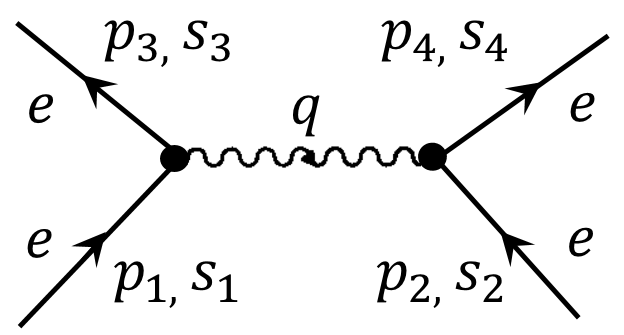
\includegraphics[width=0.45\textwidth]{figures/theory/feynman_scatter_ee_1.png}
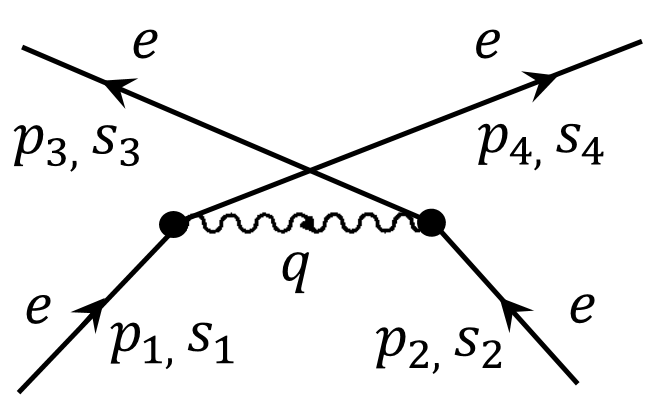
\includegraphics[width=0.45\textwidth]{figures/theory/feynman_scatter_ee_2.png}
\caption{The two lowest-order Feynman diagrams for electron electron scattering process.}
  \label{fig:feynman_scatter_ee}
 \end{center}
\end{figure}

\begin{equation}
\begin{split}
&(2\pi)^{4}\int[\bar{u}^{(s_{3})}(p_{3})(ig_{e}\gamma^{\mu})u^{(s_{1})}(p_{1})]\frac{-ig_{\mu\nu}}{q^{2}}[\bar{u}^{(s_{4})}(p_{4})(ig_{e}\gamma^{\nu})u^{(s_{2})}(p_{2})] \\
&*\delta^{4}(p_{1}-p_{3}-q)\delta^{4}(p_{2}+q-p_{4})d^{4}q
\end{split}
\label{eq:Feynman_1_6_ee_1}
\end{equation}
After do the integration and using Feynman rule 7 it gives the $\mathcal{M}$ for left plot in figure \ref{fig:feynman_scatter_ee} which is shown in \ref{eq:Feynman_7_ee_1}.
\begin{equation}
\mathcal{M}=-\frac{g_{e}^{2}}{(p_{1}-p_{3})^{2}}[\bar{u}^{(s_{3})}(p_{3})\gamma^{\mu}u^{(s_{1})}(p_{1})][\bar{u}^{(s_{4})}(p_{4})\gamma_{\mu}u^{(s_{2})}(p_{2})]
\label{eq:Feynman_7_ee_1}
\end{equation}
Similar we can get the $\mathcal{M}$ for the right plot in figure \ref{fig:feynman_scatter_ee} which is shown in \ref{eq:Feynman_7_ee_2}
\begin{equation}
\mathcal{M}=-\frac{g_{e}^{2}}{(p_{1}-p_{4})^{2}}[\bar{u}^{(s_{4})}(p_{4})\gamma^{\mu}u^{(s_{1})}(p_{1})][\bar{u}^{(s_{3})}(p_{3})\gamma_{\mu}u^{(s_{2})}(p_{2})]
\label{eq:Feynman_7_ee_2}
\end{equation}
According Feynman rule 8 these two diagrams need to be subtracted because the only difference between these two diagrams is the interchange of two outgoing electrons, it doesn't matter which diagram subtract which diagram because $|\mathcal{M}|^{2}$ is used ultimately. Finally we get the $\mathcal{M}$ for lowest-order (or tree level) of electron electron scattering process which is shown in \ref{eq:amplitude_ee}.
\begin{equation}
\mathcal{M}=-\frac{g_{e}^{2}}{(p_{1}-p_{3})^{2}}[\bar{u}(3)\gamma^{\mu}u(1)][\bar{u}(4)\gamma_{\mu}u(2)]+\frac{g_{e}^{2}}{(p_{1}-p_{4})^{2}}[\bar{u}(4)\gamma^{\mu}u(1)][\bar{u}(3)\gamma_{\mu}u(2)]
\label{eq:amplitude_ee}
\end{equation}

Until now we only consider to tree level of the electron electron scattering process, but if we add the high order contributions like one loop in the photon propagator (left plot of figure \ref{fig:screened_QED}), the result will be infinite. In order to remove this divergence, a method called "renormalization" is used which absorb the infinities into "renormalized" masses and coupling constant. For example transfer the $g_{e}=e_{bare}\sqrt{4\pi/\hbar c}$ to $g_{R}=e_{eff}\sqrt{4\pi/\hbar c}$ which means when consider the high order effect we should use the effective charge of an electron not the original charge (or the bare charge), this is because of vacuum polarization effect which behaviours like an electron virtually emits photons and the photons produce electron-positron pairs and those pairs emit further photons and so on which is shown in right plot of figure \ref{fig:screened_QED}. Hence, an electron turns out to be surrounded by many virtual electrons and positrons and due to Coulomb attractive force, positrons become closer to the original electron and thus the vacuum is polarized. Besides the effective charge will be changed by the momentum transferred $q$ in the collision, higher momentum transfer means more closer between two collided particles and higher effective charge for each particle. So the coupling $g_{R}$ is changing with $q$ and is called "running" coupling constant. However, the change of $g_{R}$ or fine structure constant ($\alpha=\frac{g_{R}^{2}}{4\pi}=\frac{e_{eff}^{2}}{\hbar c}$) versus $q$ is very small which is shown in right plot of figure \ref{fig:running_QED}.
\begin{figure}[h!]
 \begin{center}
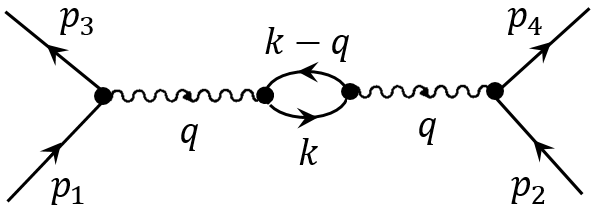
\includegraphics[width=0.45\textwidth]{figures/theory/QED_loop.png}
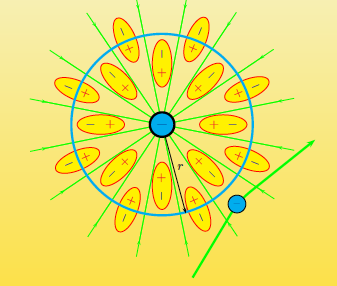
\includegraphics[width=0.35\textwidth]{figures/theory/screened.png}
\caption{The representation of the Feynman diagram with one loop in the photon propagator (left) and the vacuum polarization phenomenon causing charge screening by virtual pairs (right) \cite{screened}.}
  \label{fig:screened_QED}
 \end{center}
\end{figure}

\begin{figure}[h!]
 \begin{center}
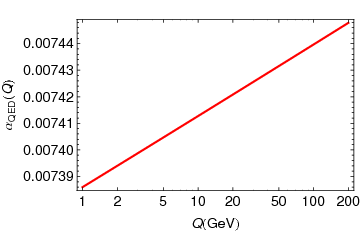
\includegraphics[width=0.45\textwidth]{figures/theory/alphaQED.png}
\caption{The momentum transfer evolution of fine structure constant $\alpha_{QED}$ \cite{Roberts:2012sv}.}
  \label{fig:running_QED}
 \end{center}
\end{figure}


\clearpage
%%%%%%%%%%%%%%%%%%% QCD%%%%%%%%%%%%%%%%%%%%%%%%%%%%%%%%%%%
\section{Quantum Chromodynamics}\label{subsec:QCD}
Here we are going to introduce some basic knowledge of Quantum Chromodynamics (QCD).
\subsection{Quark color}\label{subsec:quark_color}
The fact of quarks have colors is supported by many experiments and a direct evidence for the species of color be to 3 comes from the $e^{+}e^{-}$ annihilations experimental result on the $R$ value which defined in \ref{eq:R_value}. The first step of $e^{+}~+~e^{-}~\rightarrow~hadrons$ is $e^{+}~+~e^{-}~\rightarrow~\gamma~\rightarrow~q~+~\bar{q}$ and the Feynaman diagram is shown in left plot of figure \ref{fig:ee_qq_hadron}. This is ordinary QED process and the same as $e^{+}~+~e^{-}~\rightarrow~\gamma~\rightarrow~\mu^{+}~+~\mu^{-}$ when we replace the mass and charge of the quark by muon's mass and charge. Using the Feynman rules in \ref{subsec:Feynman_QED} we can finally get the cross section of $e^{+}~+~e^{-}~\rightarrow~\gamma~\rightarrow~q~+~\bar{q}$ or $e^{+}~+~e^{-}~\rightarrow~\gamma~\rightarrow~\mu^{+}~+~\mu^{-}$ which is shown in \ref{eq:ee_XS} when the energy of electron is substantially above the threshold ($E_{e}~>~Mc^{2}~\gg~m_{e}c^{2},~M~\mathrm{is~the~mass~of~quark~or~muon}$). The second step of $e^{+}~+~e^{-}~\rightarrow~hadrons$ is called "hadronization" which means when the two produced quarks fly away and reach a separation distance of around $10^{-15}$ m (the diameter of a hadron) the strong interaction becomes so great that new quark-antiquark pairs are produced which mainly from gluons and the phenomenon is shown in right plot of figure \ref{fig:ee_qq_hadron}.

\begin{equation}
R=\frac{\sigma(e^{+}e^{-}\rightarrow hadrons)}{\sigma(e^{+}e^{-}\rightarrow \mu^{+}\mu^{-})}
\label{eq:R_value}
\end{equation}

\begin{figure}[h!]
 \begin{center}
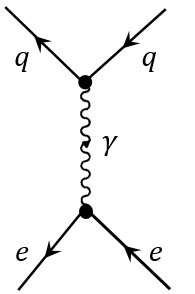
\includegraphics[width=0.25\textwidth]{figures/theory/feynman_ee_qq.png}
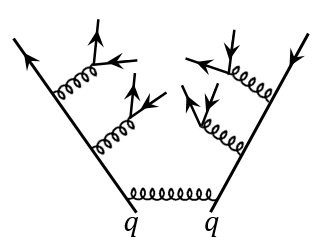
\includegraphics[width=0.45\textwidth]{figures/theory/feynman_hadronic.png}
\caption{The Feynman diagram for $e^{+}~+~e^{-}~\rightarrow~\gamma~\rightarrow~q~+~\bar{q}$ process (left). The representation of the hadronization phenomenon for quarks (right).}
  \label{fig:ee_qq_hadron}
 \end{center}
\end{figure}

\begin{equation}
\sigma=\frac{\pi}{3}(\frac{\hbar Qc\alpha}{E})^{2}
\label{eq:ee_XS}
\end{equation}

Putting equation \ref{eq:ee_XS} into \ref{eq:R_value}, it gives $R=\sum{q}e_{q}^{2}$, where the $e_{q}$ is the electric charge of the quark $q$ in quarks pairs produced in the $e^{+}e^{-}$ annihilation. Beyond the $s$ quark pair production threshold but lower then $c$ quark pair production threshold, only $u,~d,~s$ quarks contribute to this ratio $R$ and yield \ref{eq:R_u_d_s}.
\begin{equation}
\begin{split}
&R=e_{u}^{2}+e_{d}^{2}+e_{s}^{2}=\frac{2}{3},~\mathrm{(without~color)} \\
&R=2,~\mathrm{(with~3~color)}
\end{split}
\label{eq:R_u_d_s}
\end{equation}
Similarly, for higher energies beyond the $c$ quark pair production threshold but lower then $b$ quark pair production threshold, the $R$ is shown in \ref{eq:R_u_d_s_c}.
\begin{equation}
\begin{split}
&R=e_{u}^{2}+e_{d}^{2}+e_{s}^{2}+e_{c}^{2}=\frac{10}{9},~\mathrm{(without~color)} \\
&R=\frac{10}{3},~\mathrm{(with~3~color)}
\end{split}
\label{eq:R_u_d_s_c}
\end{equation}
And for more higher energies beyond the $b$ quark pair production threshold but lower then $t$ quark pair production threshold, the $R$ is shown in \ref{eq:R_u_d_s_c_b}.
\begin{equation}
\begin{split}
&R=e_{u}^{2}+e_{d}^{2}+e_{s}^{2}+e_{c}^{2}+e_{b}^{2}=\frac{11}{9},~\mathrm{(without~color)} \\
&R=\frac{11}{3},~\mathrm{(with~3~color)}
\end{split}
\label{eq:R_u_d_s_c_b}
\end{equation}
The experimental result prefer the 3 colors for any case.
\subsection{Parton distribution function}\label{subsec:pdf}

\subsection{Feynman rules for chromodynamics}\label{subsec:Feynman_QCD}
For strong interaction the coupling is $g_{s}~=~\sqrt{4\pi\alpha_{s}}$ which is similar with the coupling of electromagnetic interaction $g_{e}~=~\sqrt{4\pi\alpha}$. In order to describe quarks, we need not only Dirac spinor $u^{(s)}(p)$ which gives its momentum and spin but also a three-element column vector $c_{i}$ which gives its color shown in \ref{eq:color_vector}.
\begin{equation}
c_{1}=\begin{pmatrix} 1 \\ 0 \\ 0 \\ \end{pmatrix}~\mathrm{for~red,~~}c_{2}=\begin{pmatrix} 0 \\ 1 \\ 0 \\ \end{pmatrix}~\mathrm{for~blue,~~}c_{3}=\begin{pmatrix} 0 \\ 0 \\ 1 \\ \end{pmatrix}~\mathrm{for~green}
\label{eq:color_vector}
\end{equation}
Usually, the quark changes color at quark gluon interaction vertex and gluon takes the difference of the color between incoming quark and outgoing quark like figure \ref{fig:color_change}.
\begin{figure}[h!]
 \begin{center}
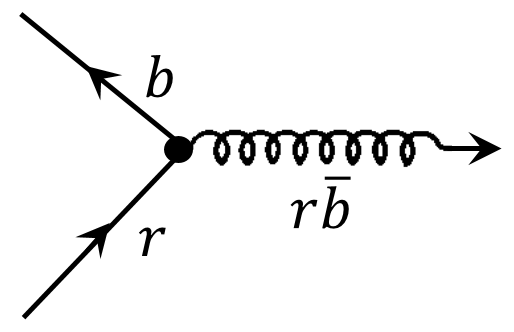
\includegraphics[width=0.45\textwidth]{figures/theory/gluon_color.png}
\caption{The representation of the quark color changes at a quark-gluon vertex.}
  \label{fig:color_change}
 \end{center}
\end{figure}
Each gluon carries one color and one anticolor, then there are nine kinds of gluons: $r\bar{r},~r\bar{b},~r\bar{g},~b\bar{r},~b\bar{b},~b\bar{g},~g\bar{r},~g\bar{b},~g\bar{g}$. In terms of color $SU(3)$ symmetry, these nine states make up a "color octet" \ref{eq:color_octet} and a "color singlet" \ref{eq:color_singlet}. If the color singlet \ref{eq:color_singlet} exist then it could be a mediator between two color singlets (e.g. a proton and a neutron) and giving rise to a long-range force with strong coupling, whereas we know the strong force is very short range. Therefore, there are evidently only eight kinds of gluons in our world.
\begin{equation}
\begin{split}
&|1\rangle=(r\bar{b}+b\bar{r})/\sqrt{2}~~~~~~~~~~|5\rangle=-i(r\bar{g}-g\bar{r})/\sqrt{2} \\
&|2\rangle=-i(r\bar{b}-b\bar{r})/\sqrt{2}~~~~~~~|6\rangle=(b\bar{g}+g\bar{b})/\sqrt{2} \\
&|3\rangle=(r\bar{r}-b\bar{b})/\sqrt{2}~~~~~~~~~~|7\rangle=-i(b\bar{g}-g\bar{b})/\sqrt{2} \\
&|4\rangle=(r\bar{g}+g\bar{r})/\sqrt{2}~~~~~~~~~~|8\rangle=(r\bar{r}+b\bar{b}-2g\bar{g})/\sqrt{2}
\end{split}
\label{eq:color_octet}
\end{equation}
\begin{equation}
|9\rangle=(r\bar{r}+b\bar{b}+g\bar{g})/\sqrt{3}
\label{eq:color_singlet}
\end{equation}
Gluons are massless particles of spin 1, liking the photon \ref{subsec:Photon} we use polarization vector $\epsilon^{\mu}$ to represent it which is orthogonal to the gluon momentum (see \ref{eq:solution_wave_photon_1}). Besides we need an eight-element column vector in order to describe the color state of the gluon shown in \ref{eq:color_column}.
\begin{equation}
a^{\alpha}=\begin{pmatrix} 1\\0\\0\\0\\0\\0\\0 \end{pmatrix}~\mathrm{for~|1\rangle~},~~~a^{\beta}=\begin{pmatrix} 0\\1\\0\\0\\0\\0\\0 \end{pmatrix}~\mathrm{for~|2\rangle~},~~~a^{\gamma}=\begin{pmatrix} 0\\0\\1\\0\\0\\0\\0 \end{pmatrix}~\mathrm{for~|3\rangle~},~~~\mathrm{and~so~on}
\label{eq:color_column}
\end{equation}


Before the statement of the Feynman rules for QCD, we need know the Gell-Mann "$\lambda$-matrices" which are shown in \ref{eq:lambda_matrices} and the commutators of the $\lambda$ matrices \ref{eq:comu_lambda} which define the "structure constants" $f^{\alpha\beta\gamma}$ of the $SU(3)$ group. The non-zero value of $f^{\alpha\beta\gamma}$ is shown in \ref{eq:structure_constant}.

\begin{equation}
\begin{split}
&\lambda^{1}=\begin{pmatrix} 0 & 1 & 0\\ 1 & 0 & 0 \\ 0 & 0 & 0 \end{pmatrix}~~~~\lambda^{2}=\begin{pmatrix} 0 & -i & 0 \\ i & 0 & 0 \\ 0 & 0 & 0 \\ \end{pmatrix}~~~~\lambda^{3}=\begin{pmatrix} 1&0&0 \\ 0&-1&0 \\ 0&0&0 \\ \end{pmatrix}\\
&\lambda^{4}=\begin{pmatrix} 0 & 0 & 1\\ 0 & 0 & 0 \\ 1 & 0 & 0 \end{pmatrix}~~~~\lambda^{5}=\begin{pmatrix} 0 & 0 & -i \\ 0 & 0 & 0 \\ i & 0 & 0 \\ \end{pmatrix}~~~~\lambda^{6}=\begin{pmatrix} 0&0&0 \\ 0&0&1 \\ 0&1&0 \\ \end{pmatrix}\\
&\lambda^{7}=\begin{pmatrix} 0 & 0 & 0\\ 0 & 0 & -i\\ 0 & i & 0 \end{pmatrix}~~~~\lambda^{8}=\begin{pmatrix} 1 & 0 & 0 \\ 0 & 1 & 0 \\ 0 & 0 & -2 \\ \end{pmatrix}
\end{split}
\label{eq:lambda_matrices}
\end{equation}

\begin{equation}
[\lambda^{\alpha},\lambda^{\beta}]=2if^{\alpha\beta\gamma}\lambda^{\gamma},~~\mathrm{here~summation~over}~\gamma~\mathrm{from~1~to~8~is~implied}
\label{eq:comu_lambda}
\end{equation}

\begin{equation}
\begin{split}
&f^{123}=1,~f^{147}=f^{246}=f^{257}=f^{345}=f^{516}=f^{637}=\frac{1}{2},\\
&f^{458}=f^{678}=\frac{\sqrt{3}}{2}
\end{split}
\label{eq:structure_constant}
\end{equation}


Similar with QED \ref{subsec:Feynman_QED} the Feynaman rules for QCD tree level (for loop diagrams it require special rules) diagrams are explained in following:

\begin{enumerate}
\item $\mathbf{Draw~the~Feynman~diagram:}$ Draw the corresponding Feynman diagrams for the process. Label four-momenta $p_{1},~p_{2},~...$ for incoming and outgoing particles together with the corresponding spins $s_{1},~s_{2},~...$. Label four-momenta $q_{1},~q_{2},~...$ for internal particles. The arrow in the line represent the direction of motion of quark or gluon, while for antiquark it is opposite with its motion.
\item $\mathbf{External~line:}$ For each external line write down $u^{(s)}(p)c$ ($\bar{u}^{(s)}(p)c^{\dag}$) for incoming (outgoing)  quark or $\bar{v}^{(s)}(p)c^{\dag}$ $(v^{(s)}(p)c)$ for incoming (outgoing) antiquark where $c$ represents the color of the correspond quark or antiquark. Besides write down $\epsilon_{\mu}(p)a^{\alpha}$ ($\epsilon_{\mu}^{\ast}(p)a^{\alpha\ast}$) for incoming (outgoing ) gluon.
\item $\mathbf{Vertex~factor:}$ Each vertex introduces a factor and there are vertex for quark-gluon or gluon-gluon interaction. Because the gluons carry color (in contrast to the photon, which is electrically neutral), they can couple with each other and there is a three-gluon vertex and a four-gluon vertex shown in figure \ref{fig:gluon_coupling}. The value of each vertex is shown in \ref{eq:QCD_vertex_factor}.

\begin{equation}
\begin{split}
&\mathrm{Quark-gluon~(left~plot~of~\ref{fig:gluon_coupling}):}~\frac{-ig_{s}}{2}\lambda^{\alpha}\gamma^{\mu} \\
&\mathrm{Three~gluon~(middle~plot~of~\ref{fig:gluon_coupling}):}~-g_{s}f^{\alpha\beta\gamma}[g_{\mu\nu}(k_{1}-k_{2})_{\lambda}+g_{\nu\lambda}(k_{2}-k_{3})_{\mu}
+g_{\lambda\mu}(k_{3}-k_{1})_{\nu}]\\
&\mathrm{,~here~the~gluon~momenta~}(k_{1},k_{2},k_{3})\mathrm{~are~assumed~to~point~into~the~vertex,}\\
&\mathrm{~if~any~point~outward,~need~change~the~sign.}\\
&\mathrm{Four~gluon~(right~plot~of~\ref{fig:gluon_coupling}):}~-ig_{s}^{2}[f^{\alpha\beta\eta}f^{\gamma\delta\eta}(g_{\mu\lambda}g_{\nu\rho}-g_{\mu\rho}g_{\nu\lambda})\\
&+f^{\alpha\delta\eta}f^{\beta\gamma\eta}(g_{\mu\nu}g_{\lambda\rho}-g_{\mu\lambda}g_{\nu\rho})+f^{\alpha\gamma\eta}f^{\delta\beta\eta}(g_{\mu\rho}g_{\nu\lambda}-g_{\mu\nu}g_{\lambda\rho})]
~~(\mathrm{summation~over}~\eta\mathrm{~implied.})
\end{split}
\label{eq:QCD_vertex_factor}
\end{equation}

\begin{figure}[h!]
\begin{center}
%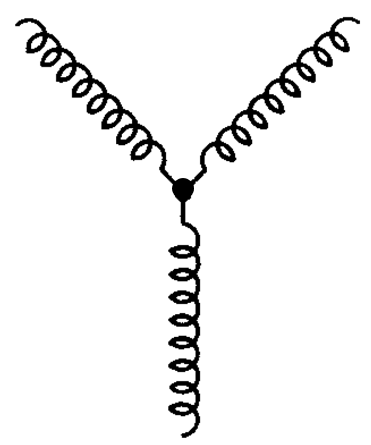
\includegraphics[width=0.3\textwidth]{figures/theory/gluon3.png}
%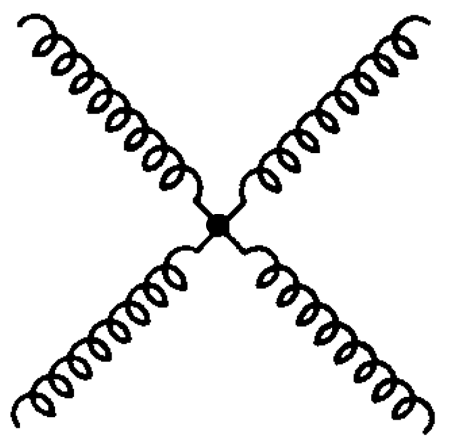
\includegraphics[width=0.35\textwidth]{figures/theory/gluon4.png}
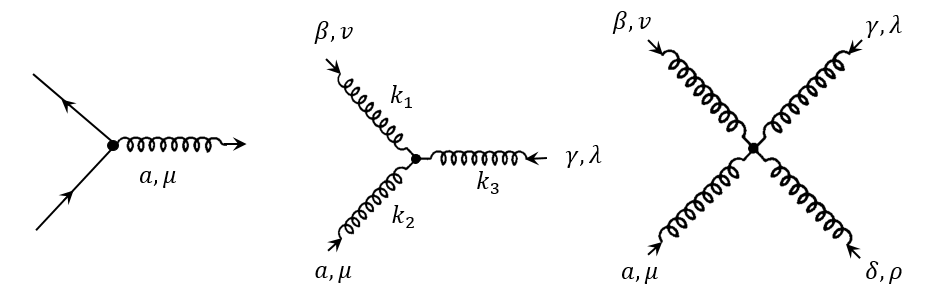
\includegraphics[width=0.9\textwidth]{figures/theory/gluon_vertex.png}
\caption{The representation of the coupling between gluons.}
\label{fig:gluon_coupling}
\end{center}
\end{figure}
\item $\mathbf{Propagator:}$ For each internal line write down a factor which is shown in \ref{eq:Feynman_Propagator}.
\begin{equation}
\begin{split}
&\mathrm{For~quark~and~antiquark~:}~~\frac{i(q\llap{/}+mc)}{q^{2}-m^{2}c^{2}},~q\llap{/}\equiv q^{\mu}\gamma_{\mu} \\
&\mathrm{For~gluon~:}~~~~~~~~~~~~~~~~~~~~~\frac{-ig_{\mu\nu}\delta^{\alpha\beta}}{q^{2}}
\end{split}
\label{eq:Feynman_Propagator}
\end{equation}
\item $\mathbf{Conservation~of~energy~and~momentum:}$ For each vertex write down a $\delta$ function with the form of $(2\pi)^{4}\delta^{4}(k_{1}~+~k_{2}~+~k_{3})$. Here the $k_{i}$ are the four-momentum of the particle which involved in the vertex, if the arrow of line $k_{i}$ is toward to the vertex then put a positive sign in front of $k_{i}$ otherwise put a negative sign (opposite for antiquark). This factor imposes the conservation of energy and momentum at each vertex, since the $\delta$ function is zero unless the sum of incoming momenta equals the sum of outgoing momenta.
\item $\mathbf{Integration~over~internal~momenta:}$ For each internal line write down a factor $\frac{1}{(2\pi)^{4}d^{4}q_{i}}$ and integrate over all internal momenta.
\item $\mathbf{Cancel~the~\delta~function:}$ Erase $(2\pi)^{4}\delta^{4}(p_{1}~+~p_{2}~+~...~+~p_{n})$ in the result which enforcing overall conservation of energy and momentum. Finally what remains is $-i\mathcal{M}$.
\item $\mathbf{Antisymmetrization:}$ Including a minus sign between diagrams which differ only in interchange of two incoming (or outgoing) quarks or antiquarks, or of an incoming quark with an outgoing antiquark (or vice versa).
\end{enumerate}

Using this Feynman rules we can calculate the $\mathcal{M}$ of the tree level QCD process. For example for $u+\bar{d}\rightarrow u\bar{d}$ process which is shown in figure \ref{fig:qqbar_scatter} it gives \ref{eq:M_qqbar} and finally the $\mathcal{M}$ is given in \ref{eq:M_qqbar1}.


\begin{figure}[h!]
\begin{center}
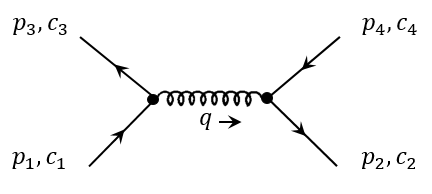
\includegraphics[width=0.45\textwidth]{figures/theory/qqbar_scatter.png}
\caption{The representation of the quark-antiquark interaction.}
\label{fig:qqbar_scatter}
\end{center}
\end{figure}

\begin{equation}
\begin{split}
&-i\mathcal{M}=[\bar{u}(3)c_{3}^{\dag}][-i\frac{g_{s}}{2}\lambda^{\alpha}\gamma^{\mu}][u(1)c_{1}][\frac{-ig_{\mu\nu}\delta^{\alpha\beta}}{q^{2}}]\\
&*[\bar{v}(2)c_{2}^{\dag}][-i\frac{g_{s}}{2}\lambda^{\beta}\gamma^{\nu}][v(4)c_{4}]
\end{split}
\label{eq:M_qqbar}
\end{equation}

\begin{equation}
\mathcal{M}=\frac{-g_{s}^{2}}{4}\frac{1}{q^{2}}[\bar{u}(3)\gamma^{\mu}u(1)][\bar{v}(2)\gamma_{\mu}v(4)](c_{3}^{\dag}\lambda^{\alpha}c_{1})(c_{2}^{\dag}\lambda^{\alpha}c_{4}), \mathrm{(summation~over~\alpha~is~implied.)}
\label{eq:M_qqbar1}
\end{equation}





\subsection{Asymptotic freedom}\label{subsec:asymptotic_freedom}
As we know for QED we using renormalization method to remove the divergence from higher level loop diagram, similar we can use it for QCD loop diagram like left plot of figure \ref{fig:QCD_loop} just thinking color as electrical charge. However, for QCD we also have virtual gluon loop which is shown in right plot of figure \ref{fig:QCD_loop}, this changes the story. It turns out that the gluon contribution works in the opposite direction which behaviours like "antiscreening" and the formula for the running coupling constant in QCD is \ref{eq:running_QCD}, where $n$ is the number of colors (3 for the Standard Model) and $f$ is the number of flavors (6 in the Standard Model). When $11n>2f$ the antiscreening effect will be dominate and the coupling will decrease with increasing $|q^{2}|$ which means at short distances the strong force becomes relatively weak and is call "asymptotic freedom". Because of the asymptotic freedom we can use perturbation theory and Feynman calculus in QCD and it is a basic ingredient in the theory of quarkonium, otherwise the Chromodynamics would have been abandoned.

\begin{figure}[h!]
 \begin{center}
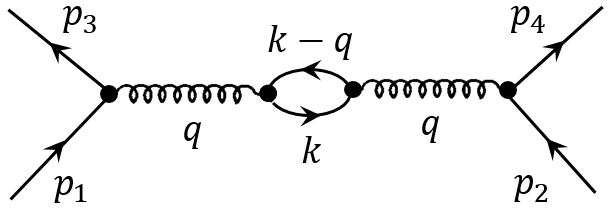
\includegraphics[width=0.45\textwidth]{figures/theory/QCD_quark_loop.png}
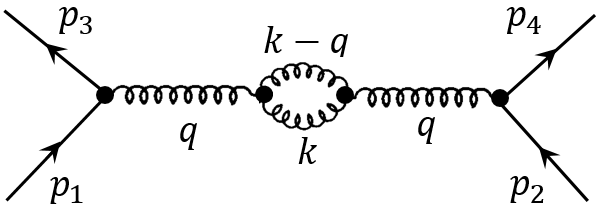
\includegraphics[width=0.45\textwidth]{figures/theory/QCD_gluon_loop.png}
\caption{The representation of the Feynman diagram with one quark-antiquark loop in the gluon propagator (left) and the Feynman diagram with one gluon-gluon loop in the gluon propagator (right).}
  \label{fig:QCD_loop}
 \end{center}
\end{figure}

\begin{equation}
\alpha_{s}(|q^{2}|)=\frac{\alpha_{s}(\mu^{2})}{1+(\alpha_{s}(\mu^{2})/12\pi)(11n-2f)\mathrm{ln}(|q^{2}|/\mu^{2})}~~(|q^{2}|\gg\mu^{2})
\label{eq:running_QCD}
\end{equation}

In order to make formula \ref{eq:running_QCD} more compact, the new variable $\Lambda$ is defined in \ref{eq:lambda}. Then the running coupling constant can be express in terms of a single parameter shown in \ref{eq:running_QCD_compact}.
\begin{equation}
\mathrm{ln}\Lambda^{2}=\mathrm{ln}\mu^{2}-12\pi/[(11n-2f)\alpha_{s}(\mu^{2})]
\label{eq:lambda}
\end{equation}

\begin{equation}
\alpha_{s}(|q^{2}|)=\frac{12\pi}{(11n-2f)\mathrm{ln}(|q^{2}|/\Lambda^{2})}~~(|q^{2}|\gg\Lambda^{2})
\label{eq:running_QCD_compact}
\end{equation}

Unfortunately, it is hard to determine $\Lambda$ precisely from experimental data, but $\Lambda c$ appears to lie somewhere in the range $100~\mathrm{MeV}<\Lambda c<500~ \mathrm{MeV}$.

Difference with the QED coupling which varies only minutely over the accessible energy range \ref{fig:running_QED}, the variation in the QCD coupling is substantial shown in figure \ref{fig:QCD_running}. When $q^{2}$ gets close to $\Lambda$ the $\alpha_{s}(|q^{2}|)$ will increase to infinite, So for the process which $q^{2}$ close to or below $\Lambda$ we have difficulty to calculate $\mathcal{M}$. Therefor for low $q^{2}$ or long-range QCD process there are a lot of work need to be done.
\begin{figure}[h!]
 \begin{center}
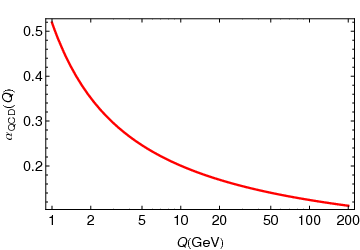
\includegraphics[width=0.45\textwidth]{figures/theory/alphaQCD.png}
\caption{The momentum transfer evolution of QCD coupling constant $\alpha_{QCD}$ \cite{Roberts:2012sv}}
  \label{fig:QCD_running}
 \end{center}
\end{figure}
\section{Weak interactions}\label{subsec:Weak}


\section{The effective field theory}\label{subsec:EFT}
\section{The Drell-Yan process}\label{subsec:DY}
\section{The shortcomings of standard model of particle physics}\label{subsec:shortcoming}
\chapter{The beyond standard model of particle physics}\label{sec:BSM}
\section{The unified ground theory}\label{subsec:GUT}
\section{The super symmetry theory}\label{subsec:SUSY}
